\chapter{The LHC-ATLAS Experiment}
\label{chap:LHCATLAS}
\section{Large Hadron Collider}
The Large Hadron Collider (LHC) is a circular collider which is located at CERN, Geneva. It was built inside the existing 27~km tunnel, previously housing the Large Electron-Positron Collider (LEP). The LHC project was planned in the 1990s and its construction started in 2000. \\
The LHC accelerates mainly protons and also heavy ions such as lead (Pb) in two beams running in opposite directions and collides them. 
The machine has been operated since 2008 and the first physics run, referred to as Run~1, was completed in 2012 with the center-of-mass energy of $\sqrt{s}$ = 7 and 8~TeV. The Higgs boson was discovered by the ATLAS and CMS experiments in 2012 \cite{HIGG-2012-27} \cite{CMS-HIG-12-028}, which was one of the most important accomplishments of this period. The energy was increased to $\sqrt{s}$ = 13~TeV for the second phase of the LHC between 2015 and 2018 referred to as Run~2. 
%The primary designed energy of the accelerator is $\sqrt{s}$ = 14~TeV.
The large amount of data provided by the LHC and its increasing in energy allowed to push the limit of our understanding of the particle physics. 

\subsection{Accelerator complex}
%pre accelerator
The particles are gradually accelerated by a chain of linear and circular accelerator complex, shown in Figure~\ref{fig:accelerator}. At first protons are in the form of hydrogen atoms. After being ionized, they are fed into the linear accelerator (LINAC~2), where they reach to the energy of 50 MeV and formed into bunches. Then they are guided to the Proton Synchrotron Booster (PSB). The PSB consists of four synchrotrons of 25~m which bring protons' energy to 1.4~GeV. The protons enter the Proton Synchrotron (PS) after that. This PS is a 638~m synchrotron and it increases the energy of the protons to 25~GeV. The final injector for the LHC is Super Proton Synchrotron (SPS), increasing the protons' energy up to 450~GeV with 7~km radius synchrotron. The SPS also provides particles for some CERN-based experiments such as AWAKE, as well as the CERN testbeam areas. \\
\begin{figure}[tbp]
\begin{center}
%\subfigure[]{
 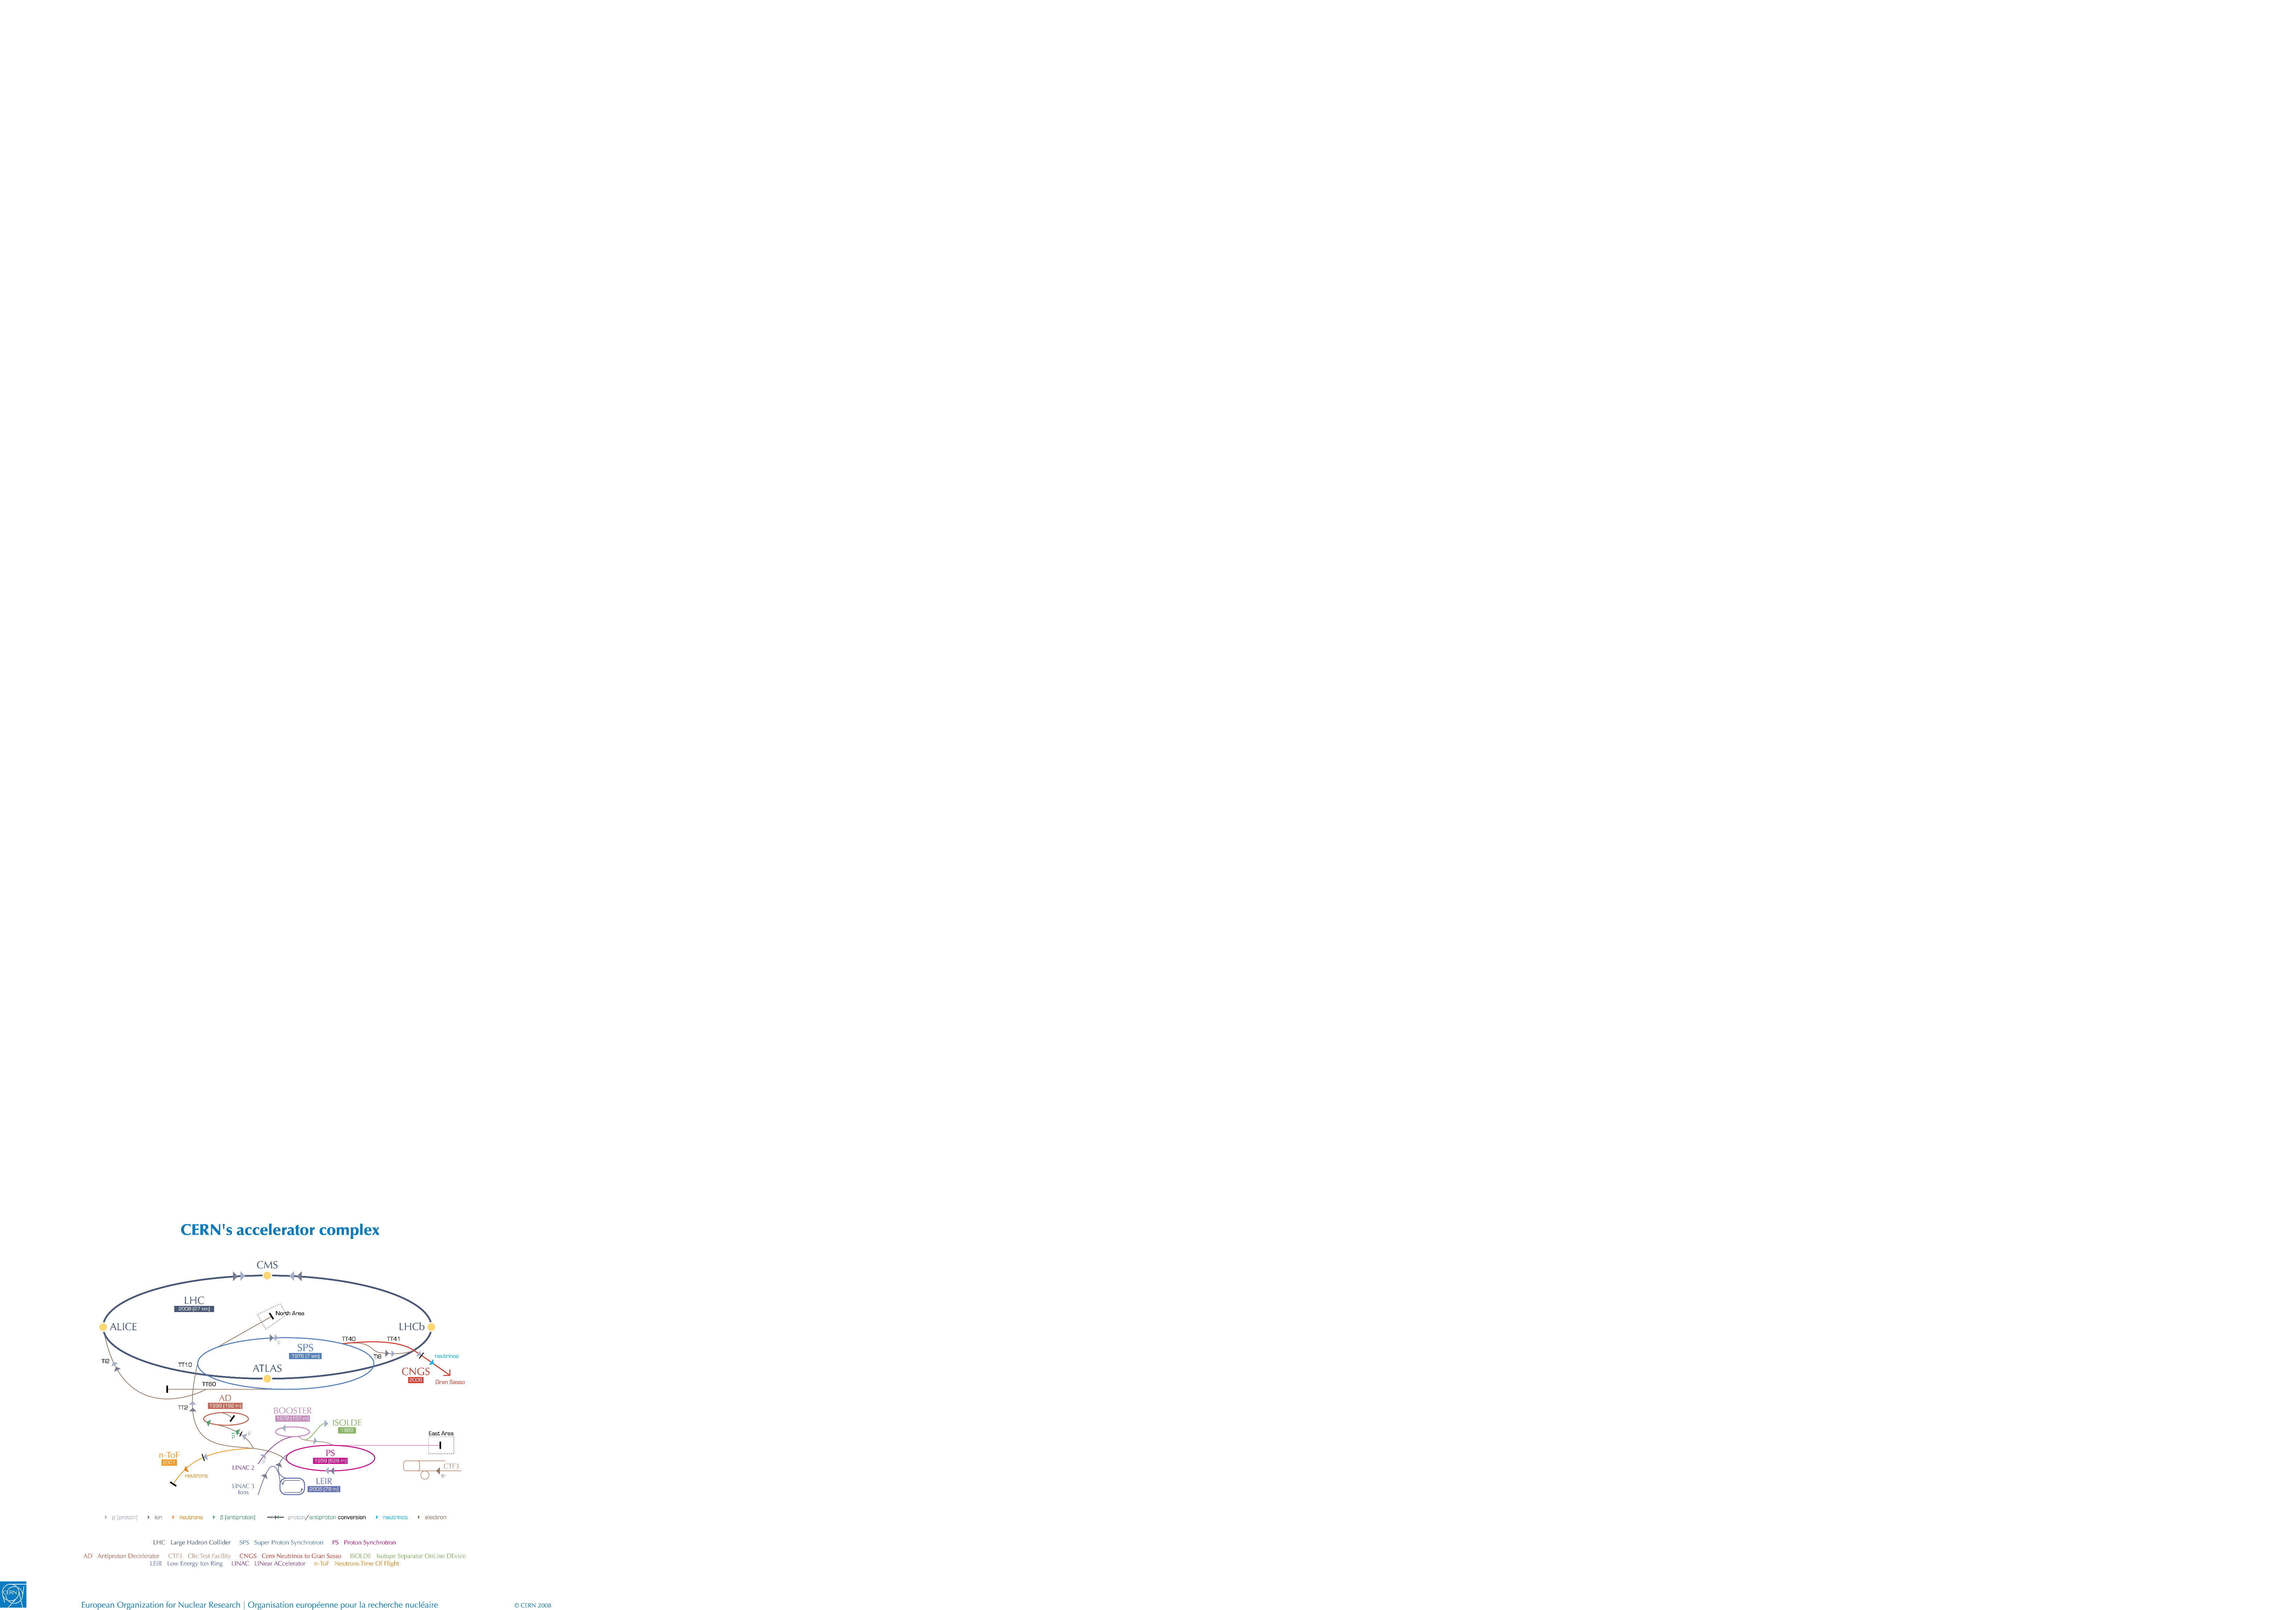
\includegraphics[width=1.1\textwidth,keepaspectratio]{figures/detector/CERN}
%}
\caption{
The whole picture of the CERN accelerator complex~\cite{accelerator} is shown. The protons are accelerated by LINAC~2, PSB, PS and SPS.
The ATLAS detector as well as the CMS, ALICE, and LHCb detectors are placed on the collision of the LHC.
}
\label{fig:accelerator}
\end{center}
\end{figure}
%electric and magnetic field
The SPS injects protons to the LHC with the energy of 450~GeV in the form of bunches, separated by 25~ns, each of which contains 1.15 $\times$ 10$^{11}$ protons. They are circulated in the two separated beam pipes. They are accelerated by an electric field while being kept curved by a magnetic field. The acceleration is performed by the eight superconducting radio frequency cavities. 
They switch the direction of the electric field at 400~MHz frequency.
They are operated at a temperature of 4.5~K. The beams are bent by the 1232 super-conducting dipole magnets to be kept in the circle trajectory. The magnetic field strength is 8.3~T, and they are operated at a temperature of 1.9~K. In addition, 392 quadruple magnets are used to focus the beams. \\
%The 4 experiments
When the protons reach the desired energy, they are collided in the experiments, at the four interaction points (IP). 
The experiments are ATLAS~\cite{PERF-2007-01}, CMS~\cite{CMS-TDR-08-001}, ALICE and LHCb. 
ATLAS and CMS are the general purpose experiments, for both the precise measurement of the SM processes and the discovery of the physics beyond the SM, ALICE is a detector dedicated to the heavy-ion collisions, which studies quark-gluon plasma, and LHCb is a forward experiment that is optimized for the heavy-flavour physics. \\
This thesis is based on the data taken by the ATLAS experiment in the Run~2 data-taking period at $\sqrt{s}$=13~TeV corresponding to an integrated luminosity of 139~fb$^{-1}$.
%\section{Luminosity}
%\label{sec:luminosity}
%The luminosity (L), the ratio of the number of events detected in a certain period of time to the cross-section is defined as:
%\begin{equation}
%L=\frac{1}{\sigma} \frac{d N}{d t}
%\end{equation}
%where $\sigma$ is the cross-section for a given proton-proton inelastic interaction process and $dN$/$dt$ is the proton-proton interaction rate.
%The luminosity is also defined with the beam parameters as:
%\begin{equation}
%L=\frac{N_1 N_2 f N_b}{4 \pi \sigma_x \sigma_y} S
%\end{equation}
%where $N_1$ and $N_2$ are the number of protons per bunch, $N_b$ is the number of bunches per fill, f is the revolution frequency of the bunches and $\sigma_x$ and $\sigma_y$ correspond to the transverse width of the beam at the collision point, the factor $S$ the geometric luminosity reduction factor to account for the crossing angle between the two beams.
%The peak instantaneous luminosity delivered to ATLAS during the year 2018 is shown in figure~\ref{fig:luminosity}. The LHC has achieved the luminosity 
\section{ATLAS Detector}
\label{sec:detector}
The ATLAS detector is a multi purpose detector, and designed to measure all standard model particles produced at the LHC.
An overview of the whole ATLAS detector is shown in Figure~\ref{fig:ATLAS}.
The ATLAS is a cylindrical detector, which is 44~m in length and 25~m in height. It consists of two areas; one is the central region, referred to as barrel region, and the other is the forward region, referred to as end-caps.
\begin{figure}[tbp]
\begin{center}
%\subfigure[]{
 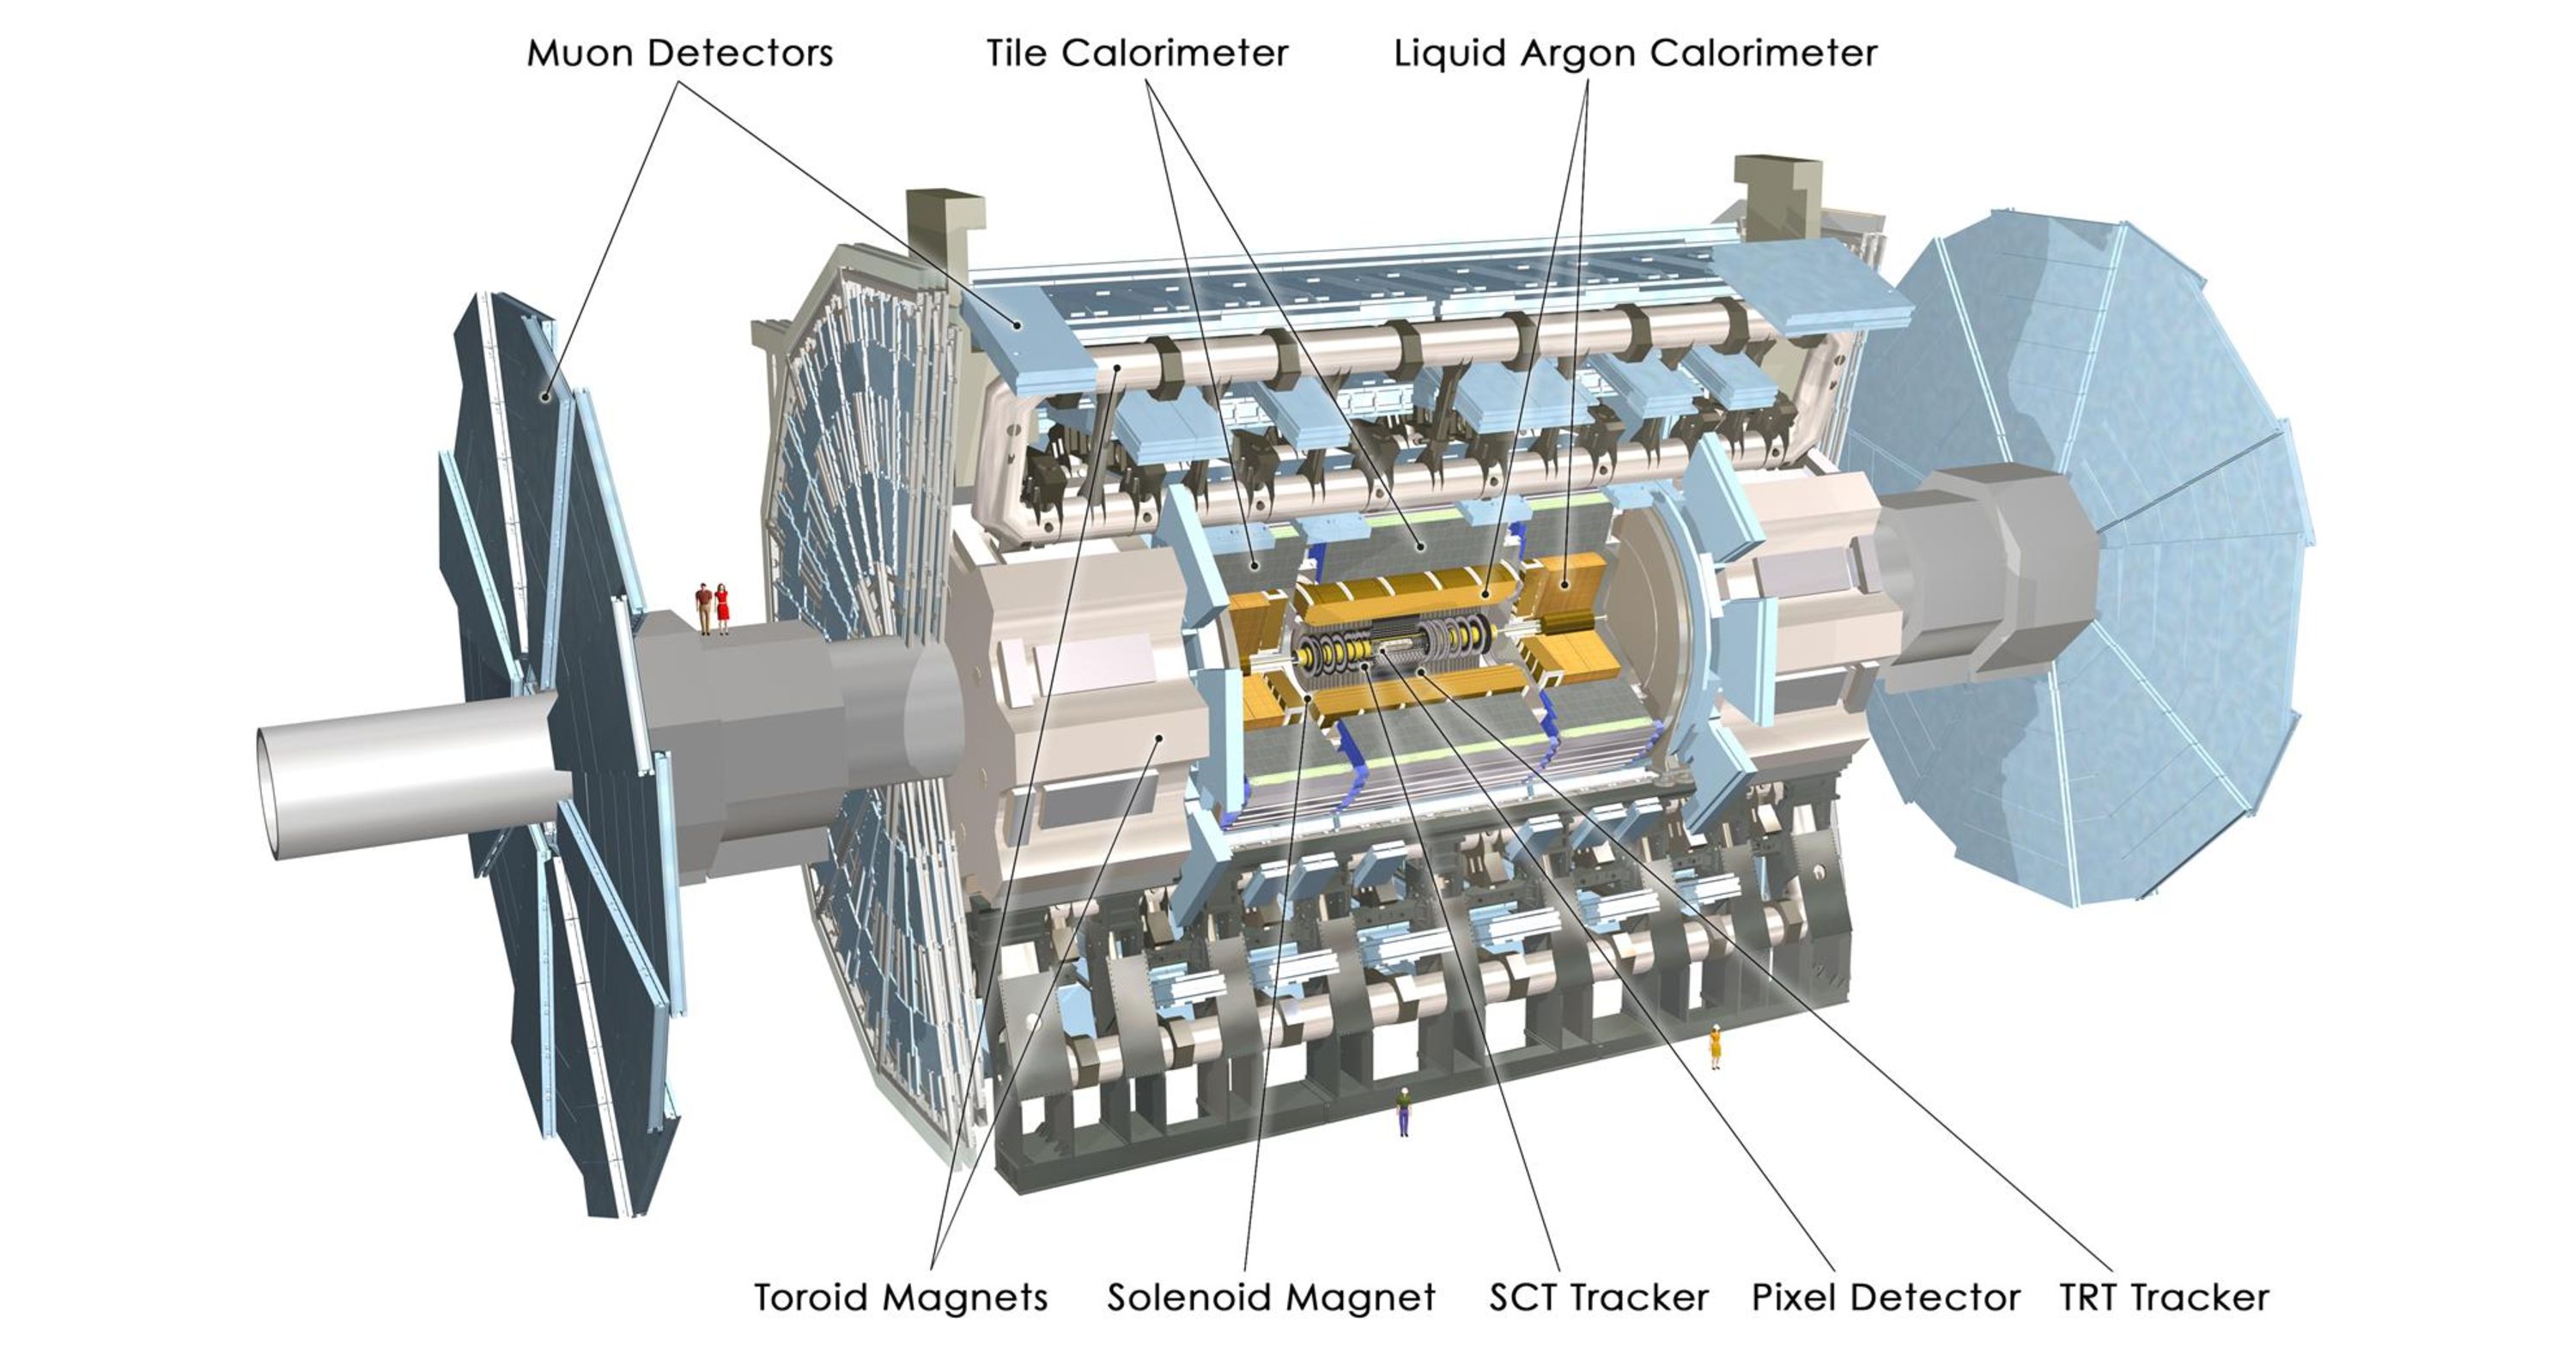
\includegraphics[width=1.0\textwidth,keepaspectratio]{figures/detector/ATLAS}
%}
\caption{
The whole picture of the ATLAS detector
}
\label{fig:ATLAS}
\end{center}
\end{figure}

\subsection{The ATLAS coordinate system}
ATLAS adopts a right-handed coordinate system with its origin at the interaction point. The z-axis is defined along the beam pipe, the y-axis points upwards and the x-axis points toward the center of the LHC. The azimuthal angle $\phi$ is the angle around the beam pipe, measured in x-y plane with respect to the x-axis. The polar angle $\theta$ is the angle to z-axis. A commonly used variable is the pseudorapidity $\eta$, which is defined as:
\begin{eqnarray*}
\eta &=& -\ln\tan(\theta/2)
\end{eqnarray*}
The low $\eta$ corresponds to the central part of the detector, while high $\eta$ region points the beam axis. At the massless limit, the difference in $\eta$ between two particles, $\Delta\eta$ is invariant under the Lorentz transformation along z-axis.
The other variable used often is the distance in the cylindrical coordinate system;
$
\Delta R = \sqrt{\Delta \eta^2 + \Delta \phi^2}
$.
Both of $\Delta \eta$ and $\Delta \phi$ are lorentz invariant, hence $\Delta R$ is also a lorentz invariant variable along z-axis.

\subsection{Magnet}
The ATLAS magnet system consists of four large superconducting magnets with a dimension of 22~m in diameter and 26~m in length with a stored energy of 1.6~GJ. A solenoid aligned on the beam axis generates 2~T axial magnetic field for the inner detector, which is placed inside the calorimeter system. 
Toroidal magnets are installed in the barrel and end-cap regions and provide 0.5 and 1~T magnetic fields for muon detectors, respectively.



There are different subsystems of the detector, the Inner Detector with the coverage of $| \eta | < 2.5$, the calorimeters with $| \eta | < 4.9$, and  the muon spectrometer with $| \eta | < 2.7$ from the inside to outside as shown in Figure~\ref{fig:ATLAS}. 
More details are described below.

\subsection{Inner Detector}
The inner detector (ID) is a tracking detector with a radius of 1.2~m and 6.2~m in length along the beam pipe. 
The ID is used for the reconstruction of the trajectory of charged particles. 
%resolution of measuring the momentum here?

The designed track momentum resolution is
\begin{eqnarray*}
    \frac{\sigma_{p_{\mathrm{T}}}}{p_{\mathrm{T}}} = 0.05~\% ~p_{\mathrm{T}}~[\mathrm{GeV}] \oplus 1~\%.
\end{eqnarray*}

The ID consists of three subsystems, Pixel, SCT, and TRT, introduced below.
The overview of the ID is shown in Figure~\ref{fig:ID}.
\begin{figure}[tbp]
\begin{center}
\subfigure{
 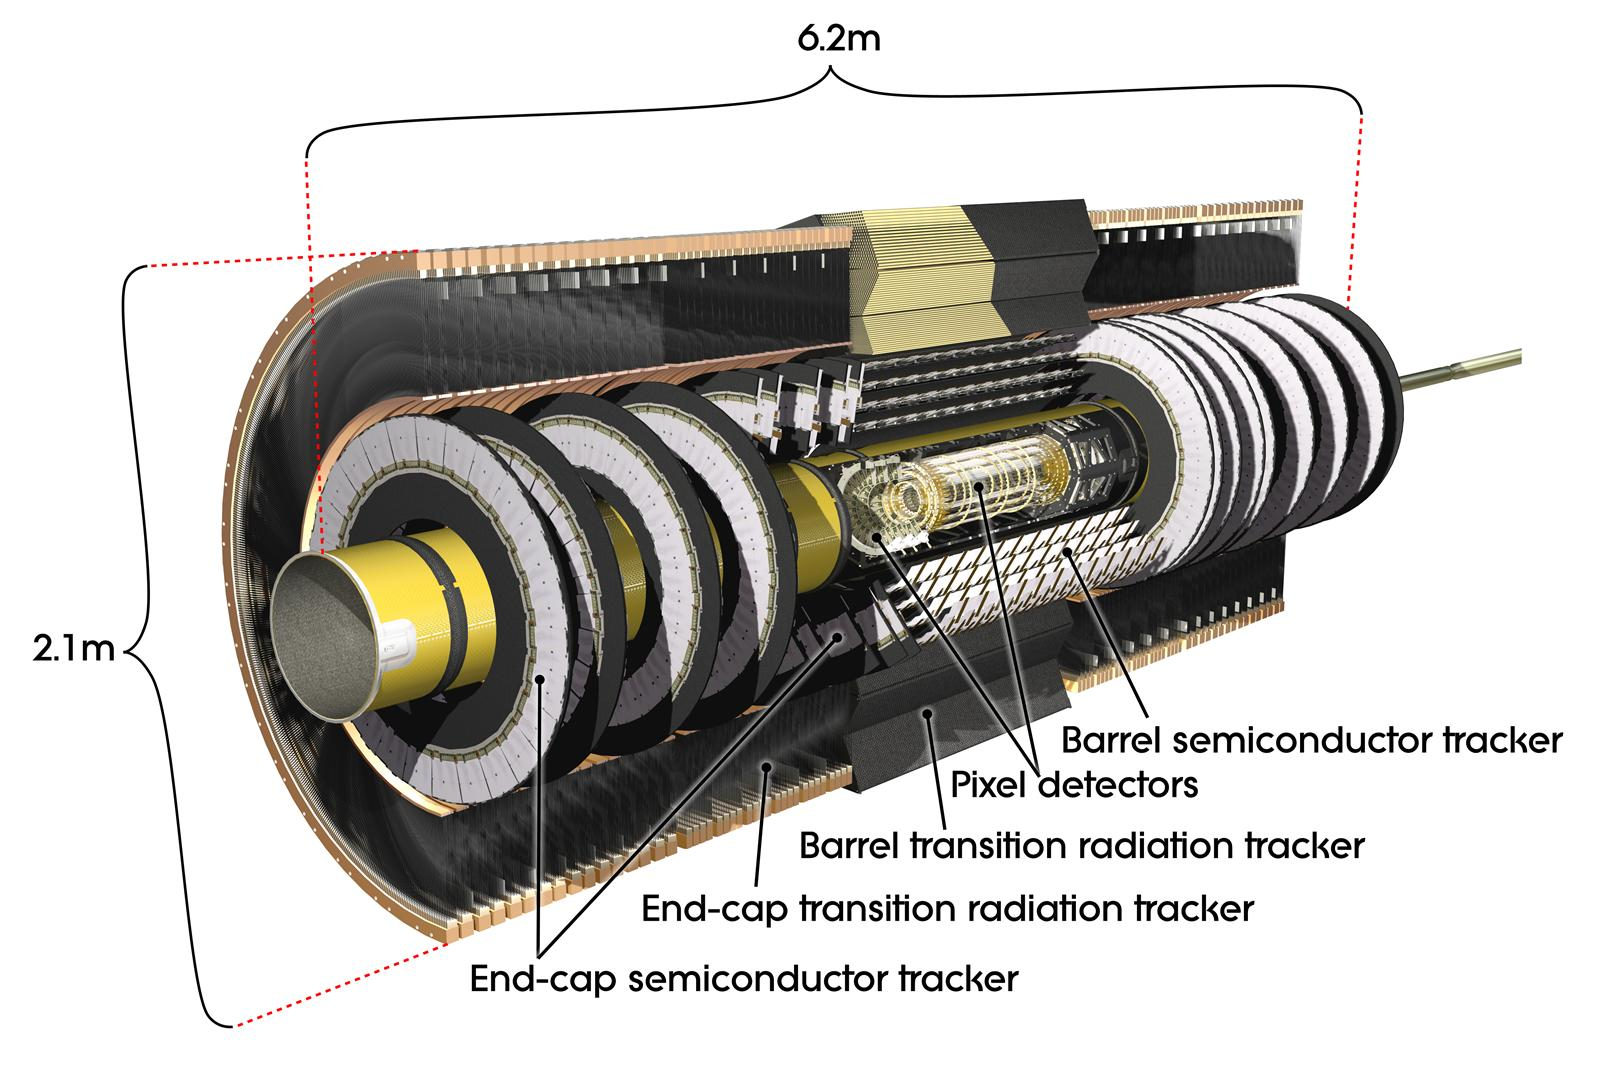
\includegraphics[width=0.8\textwidth,keepaspectratio]{figures/detector/ID2}
}
\subfigure{
 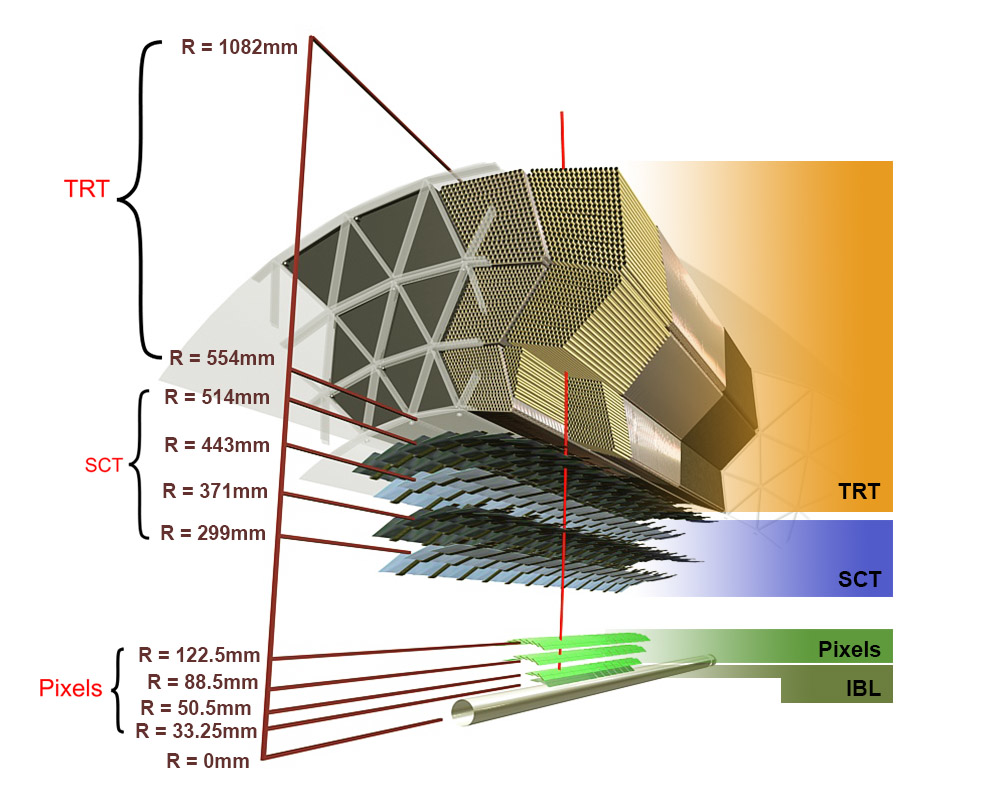
\includegraphics[width=0.7\textwidth,keepaspectratio]{figures/detector/ID1}
}
\caption{
The whole picture of the ID in section.
}
\label{fig:ID}
\end{center}
\end{figure}

\subsubsection{Pixel Detector}
The Pixel Detector covers the most inner layers of the ID system in a radius of 3~cm to 12~cm, and $|\eta|$ < 2.5. 
It consists of four cylindrical layers of silicon (Si) pixel modules.
%IBL
The innermost layer is called Insertable B-Layer (IBL), which is newly installed before the 2015 run~\cite{PIX-2018-001}. 
The IBL was inserted for ensuring a better quality of the track and vertex reconstruction, including the improvement of reconstructing the secondary vertex.
The IBL uses specifically radiation hard pixel sensors with a size of 50~$\mu m \times$ 250$\mu m$ to deal with the increasing luminosity and the radiation damage of the existing systems. 
Surrounding the IBL there are three layers with 1744 pixel sensors with a size of 50~$\mu m \times$ 400~$\mu m$. 
The layer next to the IBL is located at R = 50.5~mm. In total there are roughly 80 million readout channels, and the high granularity provides a track reconstruction with a resolution of 14~$\mu m  \times$ 115~$\mu m$.

\subsubsection{SCT}
The Semiconductor Tracker(SCT) surrounds the Pixel Detector and is located at about 30 to 50~cm from the beamline. 
It consists of silicon microstrip modules in 4 barrel layers and 9 end-cap disks.
The modules in the barrel have two layers that are slightly rotated each other. This layout allows the 2-dimensional measurement, which is the determination of the position along the strips. There are 2112 modules on the barrel and 1976 modules in the end-cap regions and the tracking resolution is about 17~$\mu$m $\times$ 580~$\mu$m.

\subsubsection{TRT}
Outside of the SCT, there is the Transition Radiation Tracker (TRT), which is located 50 to 100~cm from the beamline, covering |$\eta$| < 2.0.
It consists of drift tubes filled with gas. The tubes have a diameter of 4~mm and length of 144~m along the beam. Gas is the  mixture of Xenon (70\%), CO2 (27\%), and Oxygen (3\%). 
In addition to the measurement of the track momentum, it is used for particle identifications. 
The amount of transition radiation, which is emitted by particles crossing the interface of two materials, heavily depends on the mass of the crossing particles. Since electrons are the lightest stable charged particles and emit the most transition radiation, the TRT can be used for the separation between electrons and pions.

\subsection{Calorimeters}
The calorimeters measure the deposited energy of particles. 
The coverage of the calorimeter extends up to $|\eta|$ = 4.9. A schematic view of the system with the various components can be seen in Figure~\ref{fig:calo}.
It consists of an electromagnetic calorimeter (ECal) ($|\eta|$ < 3.2) and a hadronic calorimeter (HCal)  ($|\eta|$ < 4.9), covering full $\phi$-range. ECal is specifically designed for the measurement of photons and electrons, and the HCal for the decays of hadronic particles. The details of each subcomponent are shown below.

\begin{figure}[tbp]
\begin{center}
%\subfigure[]{
 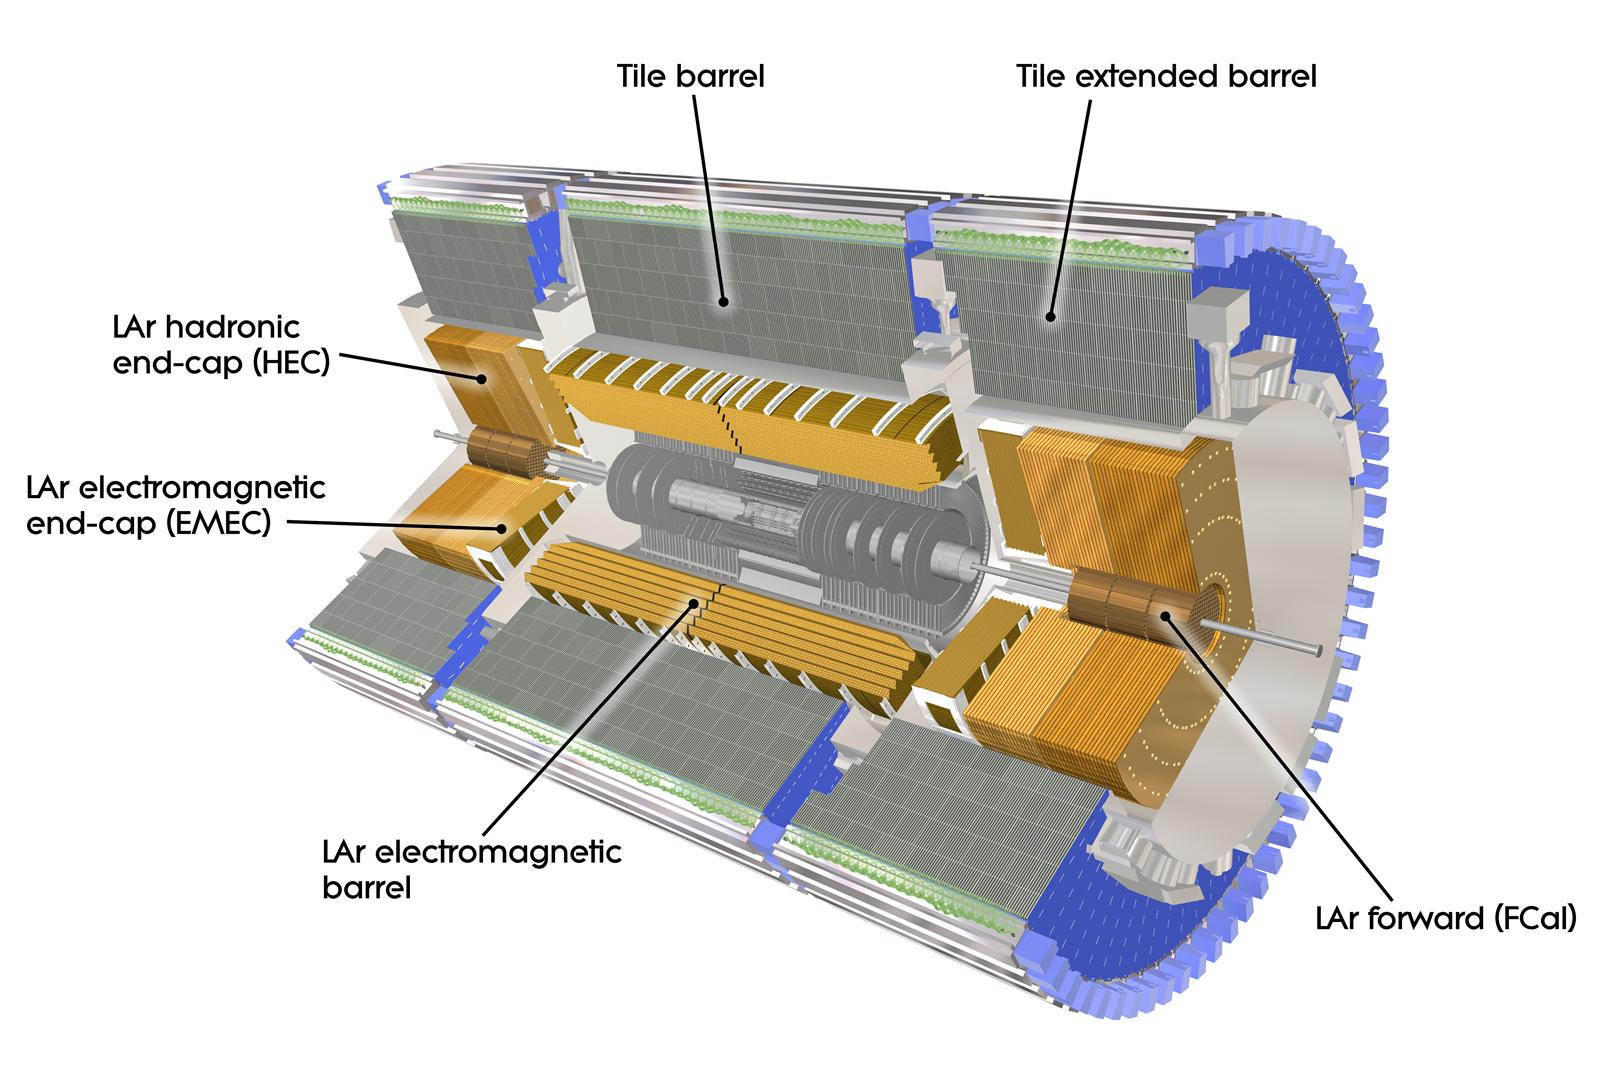
\includegraphics[width=0.8\textwidth,keepaspectratio]{figures/detector/Calo}
%}
\caption{
The whole picture of the Calorimeter with electromagnetic and hadronic subcomponents
}
\label{fig:calo}
\end{center}
\end{figure}


\subsubsection{ElectroMagnetic Calorimeter}
ECal measures the electromagnetic showers, initiated by electrons or photons. It is a sampling calorimeter using liquid Argon (LAr) with the lead (Pb) absorbers. They are arranged in an accordion geometry, which enables to cover the full $\phi$-range without azimuthal gaps. It is divided into barrel region ($|\eta|$ < 1.4) and end-caps (1.4 < $|\eta|$ < 3.2). The end-caps are divided into a central region (1.375 < $|\eta|$ < 2.5) with finer granularity and a forward region (2.5 < $|\eta|$ < 3.2) with a coarser granularity. The designed energy resolution is $\delta$E/E = 10\% $\sqrt{E/GeV} \oplus$ 0.7\%.

\subsubsection{Hadron Calorimeter}
The HCal is placed outside of the ECal to detect the hadronic shower made by hadrons.
It is divided into the barrel($|\eta|$ < 1.7), and end-caps (1.5 < $|\eta|$ < 3.2) regions. 
The barrel region is called the tile calorimeter and uses scintillating tiles with the steel absorber. 
The end-caps use LAr as detector material with copper absorber. 
The designed resolution of the hadronic in the coverage of HCal is $\delta$E/E = 50\% $\sqrt{\mathrm{E/GeV}} \oplus$ 3\%.

\subsubsection{Forward Calorimeter}
The Forward Calorimeter (FCAL) measure the energy of both electromagnetic and hadronic particles in the forward region (3.1< $|\eta|$ < 4.9)
It has three layers of absorber material. The first one is copper, optimized for electromagnetic measurements and the other two are made of tungsten for hadronic measurements. 
The design resolution of the forward calorimeter for jets is $\delta$E/E = 100\% $\sqrt{\mathrm{E/GeV}} \oplus$ 10\%.

\subsection{Muon Spectrometer}
The Muon Spectrometer (MS) is placed on the most outside of the ATLAS detector to identify muons and to make a precise estimation of their transverse momentum.
%Muons are the Minimum Ionizing Particles for a large energy range, they cross the calorimeters without being absorbed, and can be measured precisely at MS. 
The coverage of the MS extends up to $|\eta|$ < 2.7. A schematic view of the whole MS is shown in Figure~\ref{fig:MS}.
It is divided into  barrel ($|\eta|$ < 1.4), end caps (1.6 < $|\eta|$ < 2.7) and
transition region (1.4 < $|\eta|$ < 1.6).

\begin{figure}[tbp]
\begin{center}
%\subfigure[]{
 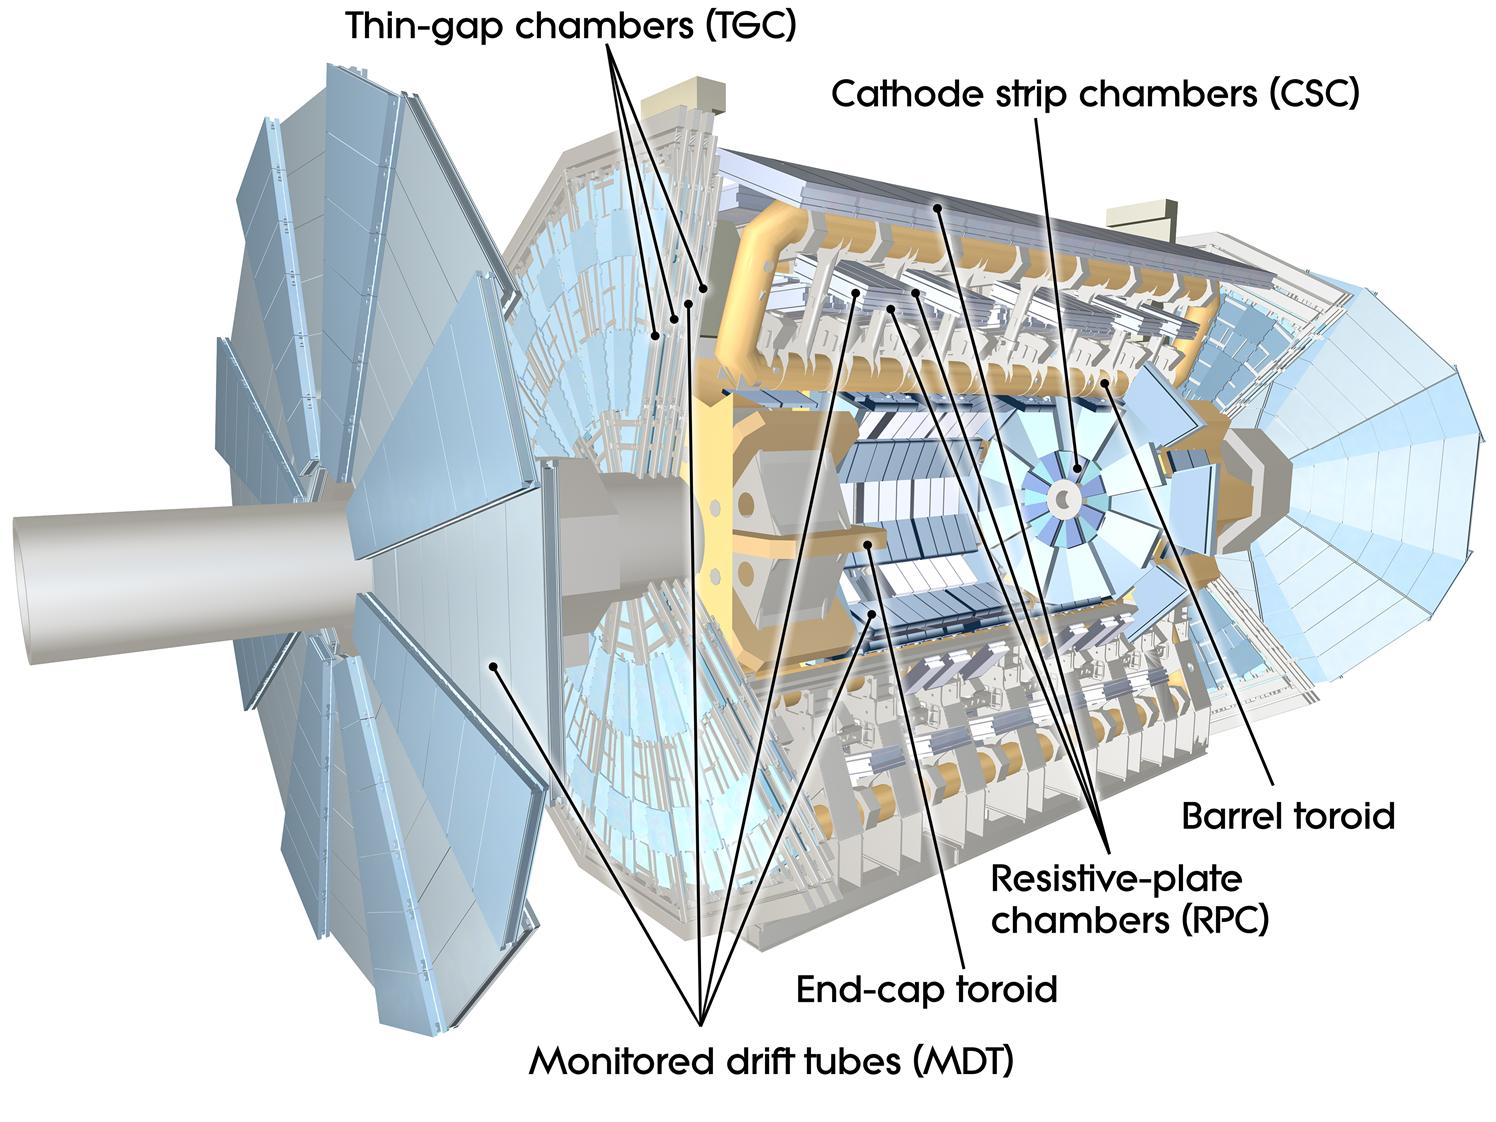
\includegraphics[width=0.8\textwidth,keepaspectratio]{figures/detector/MS}
%}
\caption{
The whole picture of the Muon Spectrometer
}
\label{fig:MS}
\end{center}
\end{figure}

The MS is an ionization detector using gas. When a charged particle crosses the active area, it ionizes the gas, and the applied electric field guides the electrons and ions to be collected. It consists of 4 sub-detectors, described below.

\subsubsection{Monitored Drift Tubes and Cathode Strip Chambers}
The Monitored Drift Tubes (MDTs) perform the precision position measurement of muons 
in $|\eta|$ < 2.7. It consists of the 30~mm diameter drift tubes filled with gas of Ar and CO$_2$ and wires operated at high voltage to collect the electrons.
The tubes are organized in layers and form chambers.

The Cathode Strip Chambers (CSCs) are multi-wire proportional chambers also filled with gas. They perform the same task as the MDTs in the forward region (2 < $|\eta|$ < 2.7), where the counting rate is rather high. 

\subsubsection{Resistive Plate Chambers and Thin Gap Chambers}
The Resistive Plate Chambers (RPCs) are installed in the barrel in  $|\eta|$ < 1.05. Single RPC consists of two resistive plates separated by a thin gas gap. They are mainly used to  provid the muon triggers for the Data Acquisition (DAQ) system.

The Thin Gap Chambers(TGCs) are also multi-wire proportional chambers similar to the CSCs. They serve the same purpose as the RPCs, but in the forward region. 

\subsection{Triggers}
The event rate provided by the LHC is around 40~MHz. It is impossible to record all the information from the detectors at such a high rate, hence the selection of the event of interest to have high-$p_\mathrm{T}$ $e$, $\mu$, $\tau$, and jets is performed with a trigger system. The layout of the ATLAS trigger system is shown in Figure~\ref{fig:Trigger}.

\begin{figure}[tbp]
\begin{center}
%\subfigure[]{
 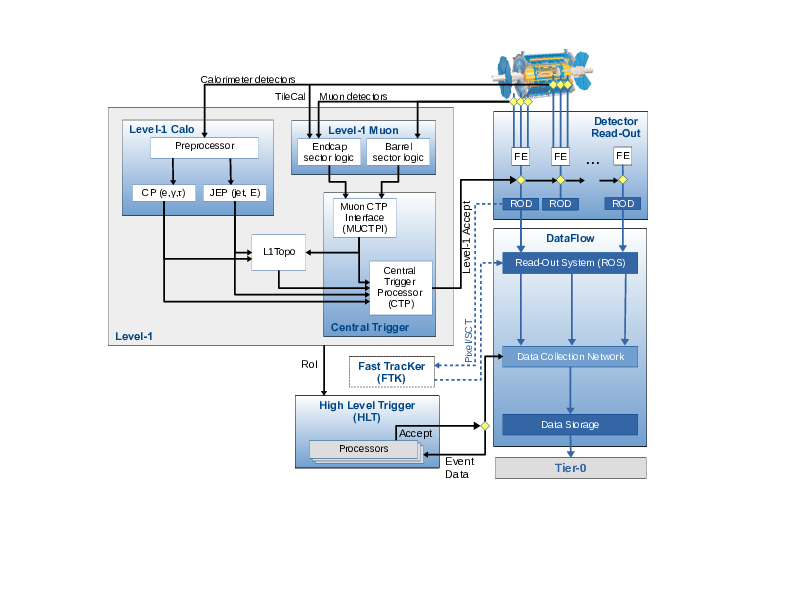
\includegraphics[width=0.8\textwidth,keepaspectratio]{figures/detector/Trigger}
%}
\caption{
The layout of the ATLAS trigger system in Run~2
}
\label{fig:Trigger}
\end{center}
\end{figure}
The ATLAS trigger system~\cite{TRIG-2019-04} consists of hardware based Level-1 (L1) trigger, and software based High Level Trigger (HLT). 
The L1 trigger is implemented with custom electronics and roughly reconstructs high-$p_\mathrm{T}$, $e/\gamma$, $\mu$, $j$, and so on to determine the Regions-of-Interest (RoIs) in the HLT algorithms, from coarse granularity calorimeter and the muon spectrometer information. 
These data are treated by sub-systems, the L1Calo and L1Muon, respectively. 
L1 electron is reconstructed by L1Calo. 2$\times$2 core towers and 12 surrounded towers of ECal are used for capturing the electron energy and calculating isolation requirement, respectively. The sketch of these calorimeter towers is shown in figure~\ref{fig:TriggerTower}.
The L1 Muon makes use of RPC and TGC hits and fires if there is a coincidence between different chambers based on the predefined look-up-tables.
The schematic of the muon barrel trigger is shown in figure~\ref{fig:muontrigger}.
The reconstructed L1 objects by the L1Calo and the L1Muon are sent to the L1Topo, and the selections based on kinematical information can be performed. 
Then all information from L1Calo, L1Muon, and the L1Topo are sent to the Central Trigger Processor (CTP). 
The L1 trigger reduces the event rate from approximately 40~MHz to 100~kHz, and the decision time of the L1 is 2.5~$\mu$s.
The RoIs decided at L1 are then sent to the HLT, which is a farm of large CPU cores.
The HLT reconstructs objects with the full detector information around the RoIs. 
It reduces the rate of the L1 output of 100~kHz to approximately 1~kHz on average, within a processing time of about 200~ms.
Events that pass the trigger selections are recorded on disk, where data can be used for further analysis off-line.
\begin{figure}[tbp]
\begin{center}
%\subfigure[]{
 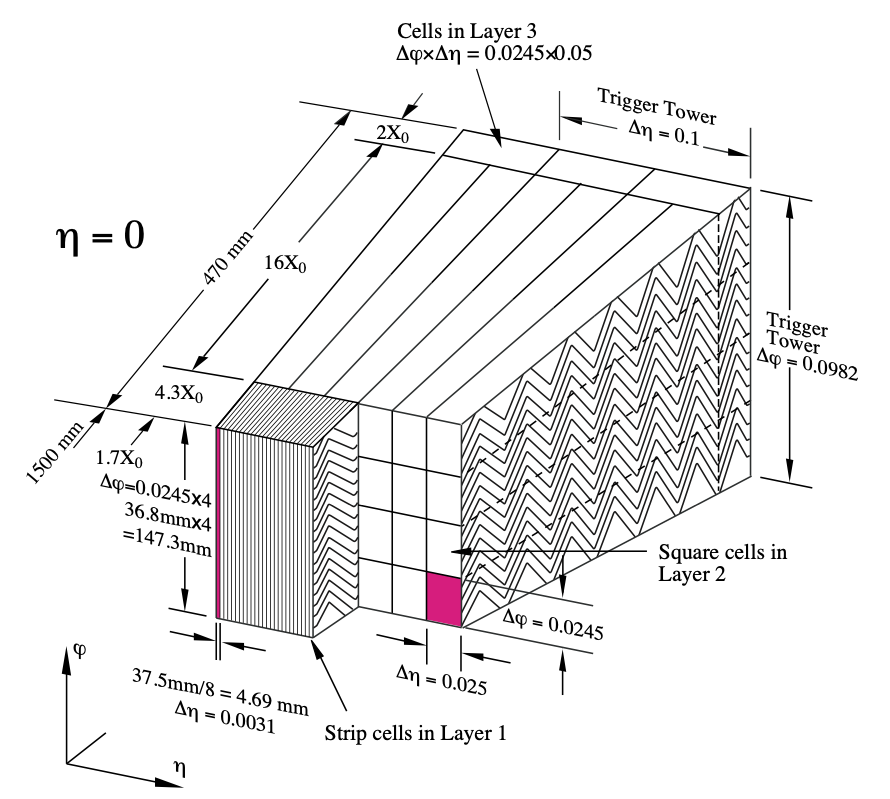
\includegraphics[width=0.6\textwidth,keepaspectratio]{figures/detector/TriggerTower}
%}
\caption{
The sketch of the barrel module of the ECal~\cite{PERF-2007-01}.
}
\label{fig:TriggerTower}
\end{center}
\end{figure}

\begin{figure}[tbp]
\centering
\begin{center}
%\subfigure[]{
 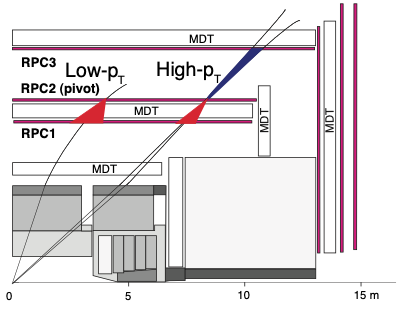
\includegraphics[width=0.5\textwidth,keepaspectratio]{figures/detector/muontrigger}
%}
\caption{
The schematic of the muon barrel trigger.~\cite{PERF-2007-01}. RPC hits are used for triggers.
}
\label{fig:muontrigger}
\end{center}
\end{figure}

